\documentclass[a4paper,14pt]{extreport}
\usepackage[T2A]{fontenc}
\usepackage[utf8x]{inputenc}%включаем свою кодировку: koi8-r или utf8 в UNIX, cp1251 в Windows
\usepackage[english,russian]{babel}%используем русский и английский языки с переносами
\usepackage{indentfirst}
\usepackage{cite,enumerate,float}
\usepackage{amsmath, amssymb}
\usepackage{graphicx}
\graphicspath{{images/},{plots/}}%путь к рисункам

\usepackage{multicol, multirow, array}
\newcolumntype{C}[1]{>{\centering\arraybackslash}m{#1\textwidth}}
\renewcommand{\arraystretch}{1.2}
\usepackage{times}
\renewcommand{\rmdefault}{ftm}

\usepackage{geometry}
\geometry{left=2cm}% левое поле
\geometry{right=1.5cm}% правое поле
\geometry{top=2cm}% верхнее поле
\geometry{bottom=2cm}% нижнее поле

\usepackage{tocloft}
\renewcommand{\cfttoctitlefont}{\normalfont}
\makeatletter
\renewcommand*\l@chapter[2]{%
  \ifnum \c@tocdepth >\z@
    \addpenalty\@secpenalty
    \addvspace{1.0em \@plus\p@}%
    \setlength\@tempdima{1.5em}%
    \begingroup
      \parindent \z@ \rightskip \@pnumwidth
      \parfillskip -\@pnumwidth
      \leavevmode
      \advance\leftskip\@tempdima
      \hskip -\leftskip
      #1\nobreak\cftdotfill{\cftdotsep} \nobreak\hb@xt@\@pnumwidth{\hss #2}\par
    \endgroup
  \fi}
\renewcommand*\l@section[2]{%
  \ifnum \c@tocdepth >\@ne
    \addpenalty\@secpenalty
    \addvspace{1.0em \@plus\p@}%
    \setlength\@tempdima{1.5em}%
    \begingroup
      \parindent \z@ \rightskip \@pnumwidth
      \parfillskip -\@pnumwidth
      \leavevmode
      \advance\leftskip\@tempdima
      \hskip -\leftskip
      #1\nobreak\cftdotfill{\cftdotsep} \nobreak\hb@xt@\@pnumwidth{\hss #2}\par
    \endgroup
  \fi}
\renewcommand*\l@subsection[2]{%
\ifnum \c@tocdepth >\tw@
  \addpenalty\@secpenalty
  \addvspace{1.0em \@plus\p@}%
  \setlength\@tempdima{1.5em}%
  \begingroup
    \parindent \z@ \rightskip \@pnumwidth
    \parfillskip -\@pnumwidth
    \leavevmode
    \advance\leftskip\@tempdima
    \hskip -\leftskip
    #1\nobreak\cftdotfill{\cftdotsep} \nobreak\hb@xt@\@pnumwidth{\hss #2}\par
  \endgroup
\fi}
\makeatother
\usepackage{setspace}

\usepackage{titlesec}
\usepackage[square, numbers, sort&compress]{natbib}
\usepackage[unicode, colorlinks, linkcolor=black,
citecolor=black,urlcolor=black]{hyperref}

\renewcommand{\arraystretch}{1.2}

\renewcommand{\small}{\fontsize{12pt}{14.4pt}\selectfont}
\usepackage{caption}
\DeclareCaptionLabelFormat{figure}{Рисунок #2}
\DeclareCaptionLabelFormat{table}{Таблица #2}
\DeclareCaptionLabelSeparator{sep}{~---~}
\captionsetup{labelsep=sep,justification=centering,font=small}
\captionsetup[figure]{labelformat=figure}
\captionsetup[table]{labelformat=table}

\renewcommand{\theenumi}{\arabic{enumi}}
\renewcommand{\labelenumi}{\arabic{enumi})}
\renewcommand{\theenumii}{.\arabic{enumii}}
\renewcommand{\labelenumii}{\arabic{enumi}.\arabic{enumii})}
\renewcommand{\theenumiii}{.\arabic{enumiii}}
\renewcommand{\labelenumiii}{\arabic{enumi}.\arabic{enumii}.\arabic{enumiii})}

\newcommand{\pder}[2] {\frac{\partial #1}{\partial #2}}
      % частная производная от #1 по #2
\newcommand{\ppder}[2]{\frac{\partial^2 #1}{\partial {#2}^2}}
  % вторая частная производная от #1 по #2
\newcommand{\pcder}[3]{\frac{\partial^2 #1}{\partial #2 \partial #3}}
  % вторая частная производная от #1 по #2 и #3
\newcommand{\der}[2]  {\frac{d #1}{d #2}}
  % производная от #1 по #2
\newcommand{\dder}[2] {\frac{d^2 #1}{d {#2}^2}}
  % вторая производная от #1 по #2

% --- обозначения и команды ---
\newcommand{\const}{\mathrm{const}}                     % константа
\newcommand{\average}[1]{\left\langle #1 \right\rangle} % обозначение среднего
\newcommand{\abs}[1]{\left| #1 \right|}                 % обозначение модуля
\newcommand{\ds}{\displaystyle}                         % полный размер строчной формулы
\newcommand{\D}{\Delta}
\newcommand{\dotunder}[1]{\d{#1}} % необходима для обозначения строчной дельты
\renewcommand{\d}{\delta}
\newcommand{\eps}{\varepsilon}
\renewcommand{\phi}{\varphi}
% xxx обозначения и команды xxx

\newcommand{\divergence}{\mathrm{div\,}}  % дивергенция
\newcommand{\gradient}  {\mathrm{grad\,}} % градиент
\newcommand{\rotor}     {\mathrm{rot\,}}  %
% title style
\titleformat{\chapter}
    {\centering\normalsize}
    {\thechapter}
    {8pt}{\MakeUppercase}
\titleformat{\section}
    {\centering\normalsize}
    {\thesection}
    {1em}{}
\titleformat{\subsection}
    {\centering\normalsize}
    {\thesubsection}
    {1em}{}

\titlespacing*{\chapter}{0pt}{-30pt}{8pt}
\titlespacing*{\paragraph}{0pt}{-30pt}{8pt}
\titlespacing*{\section}{\parindent}{*4}{*4}
\titlespacing*{\subsection}{\parindent}{*4}{*4}

\makeatletter

\renewcommand{\@biblabel}[1]{#1}

% bibliography bibitem item indent
\renewenvironment{thebibliography}[1]
    {\chapter*{\bibname}%
    \@mkboth{\MakeUppercase\bibname}{\MakeUppercase\bibname}%
    \list{\@biblabel{\@arabic\c@enumiv}}%
        {\settowidth\labelwidth{\@biblabel{#1}}%
        \leftmargin=0pt
        \itemindent=50pt
        \@openbib@code
        \usecounter{enumiv}%
        \let\p@enumiv\@empty
        \renewcommand\theenumiv{\@arabic\c@enumiv}}%
    \sloppy
    \clubpenalty4000
    \@clubpenalty \clubpenalty
    \widowpenalty4000%
    \sfcode`\.\@m}
        {\def\@noitemerr
        {\@latex@warning{Empty `thebibliography' environment}}%
    \endlist}

\makeatother

\newcolumntype{C}[1]{>{\centering\arraybackslash}m{#1\textwidth}}
\renewcommand{\arraystretch}{1.2}

\DeclareCaptionLabelFormat{figure}{Рисунок #2}
\DeclareCaptionLabelFormat{table}{Таблица #2}
\DeclareCaptionLabelSeparator{sep}{~---~}
\captionsetup{labelsep=sep, justification=centering, font=small}
\captionsetup[figure]{labelformat=figure}
\captionsetup[table]{labelformat=table}

\renewcommand{\cfttoctitlefont}{\normalfont\hspace{0.38\textwidth}}
\renewcommand{\cftbeforetoctitleskip}{-1em}
\renewcommand{\cftchapfont}{\normalsize}
\renewcommand{\cftsecfont}{\hspace{-21pt}}
\renewcommand{\cftsubsecfont}{\hspace{-53pt}}
\renewcommand{\cftbeforechapskip}{0em}
\renewcommand{\cftparskip}{-1mm}
\renewcommand{\cftdotsep}{1}
\renewcommand{\cftsecpresnum}{}
\renewcommand{\cftchapleader}{\cftdotfill{\cftdotsep}}
\renewcommand{\cftsecleader}{\cftdotfill{\cftdotsep}}
\renewcommand{\cftsecaftersnum}{.}
\renewcommand{\cftsubsecaftersnum}{.}
\setcounter{tocdepth}{2}

\renewcommand{\theenumi}{\arabic{enumi}}
\renewcommand{\labelenumi}{\arabic{enumi})}
\renewcommand{\theenumii}{.\arabic{enumii}}
\renewcommand{\labelenumii}{\arabic{enumi}.\arabic{enumii})}
\renewcommand{\theenumiii}{.\arabic{enumiii}}
\renewcommand{\labelenumiii}{\arabic{enumi}.\arabic{enumii}.\arabic{enumiii})}

\begin{document}
\onehalfspacing
\setlength{\parindent}{1.25cm}
\setcounter{page}{4}
\begin{center}
РЕФЕРАТ
\end{center}
Целью данной работы является получение уравнений, описывающих воздействие
СВЧ-излучения на ионные токи в клеточных мембранах. В ходе работы на основе
уравнений Нернста-Планка и Пуассона получены уравнения для нестационарных
процессов в мембранах. Применение этих уравнений для внешних периодических
возмущений позволило получить уравнения для поля в мембране, находящейся во
внешнем СВЧ-поле.
\vspace*{1cm}

\noindent Ключевые слова: мембранный транспорт, СВЧ-излучение,
электродиффузия, уравнение Нернста-Планка, уравнение Пуассона, теория
возмущений, нестационарный процесс.
\vspace*{1cm}

\begin{center}
    ABSTRACT
\end{center}

The purpose of this work is to obtain the equations describing the effects of
microwave radiation on the ionic currents in cell membranes. During the work
on the basis of the equation Nernst-Planck and Poisson equations are derived
for non-stationary processes in membranes. The use of these equations for the
external periodic perturbation yielded field equations in the membrane in an
external microwave field.
\vspace*{1cm}

\noindent Key words: membrane transport, microwaves, electrodiffusion,
Nernst-Planck equation, Poisson equation, perturbation theory,
non-stationary process.

\newpage
\renewcommand{\contentsname}{\begin{center}СОДЕРЖАНИЕ\end{center}}
\tableofcontents
\newpage
\begin{center}
    ОПРЕДЕЛЕНИЯ, ОБОЗНАЧЕНИЯ И СОКРАЩЕНИЯ
\end{center}

\newpage
\begin{center}
    ВВЕДЕНИЕ
\end{center}
\addcontentsline{toc}{chapter}{Введение}
\vspace*{1cm}

\newpage
\chapter{Уравнение Нернста--Планка}
\section{Основные положения}

Если считать мембрану гомогенной средой, в которой может происходить диффузия и
миграция ионов, парциальный электрический ток ионов сорта к можно записать в
виде \cite{bib:8}:
\begin{equation}
    I_k = -\frac{z_k}{\abs{z_k}}u_kRT\pder{c_k}{x} + \abs{z_k}u_kc_kFE,
    \label{eq:nernst-plank}
\end{equation}
где \( z_k \) -- заряд иона сорта к (в единицах заряда протона), \( u_k \) --
подвижность, Е -- напряженность электрического поля.
Суммарная плотность ионного тока определяется как сумма
\[
    I = \sum_{k=1}^n I_k.
\]
В стационарном случае парциальные токи сохраняются, так что \( I_k = \const \),
и соотношение \eqref{eq:nernst-plank} представляет собой нелинейное
дифференциальное уравнение первого порядка, содержащее неизвестные функции
\( c_k \) и \( E \) и неизвестную постоянную \( I_k \). Это основное
электродиффузионное уравнение носит название уравнения Нернста -- Планка
\cite{bib:16}.
Если рассматриваемая система содержит \( n \) сортов ионов, то мы имеем \( n \)
уравнений \eqref{eq:nernst-plank} для \( n + 1 \) функций, в число которых
входят все \( c_k \) и \( Е \). Чтобы сделать задачу определенной, необходимо
располагать еще одним уравнением. Таким уравнением служит уравнение Пуассона.
Ввиду важности выпишем систему уравнений электродиффузионной задачи:
\begin{equation}
\left\{
    \begin{array}{l}
        \ds \der{c_k}{x} - \beta z_k c_k e E =
            - \frac{I_k\abs{z_k}}{z_k u_k RT},\\
        \ds \der{E}{x} = \frac{F}{\eps\eps_0}\sum_{k=1}^n z_k c_k.
    \end{array}
\right.
\label{eq:system_nernst-plank}
\end{equation}
Задавая \( 2n + 2 \) граничных условий, мы получаем окончательную постановку
проблемы.

Кроме дифференциальной формулировки электродиффузионных уравнений
\eqref{eq:nernst-plank} и \eqref{eq:system_nernst-plank} иногда оказывается
полезной интегральная. Проинтегрируем уравнение Пуассона от некоторой точки
\( \overline{x} \) до \( x \) \cite{bib:8}:
\begin{equation}
    E(x, t) = E(\overline{x}, t) + \frac{F}{\eps}\sum_{k=1}^n z_k
    \int_{\overline{x}}^x c_k(x', t) dx'.
    \label{eq:electric_field}
\end{equation}
Подставляя \eqref{eq:electric_field} в выражение для разности потенциалов на мембране
\[
    \phi(t) = -\int_0^\delta E(x', t) dx',
\]
получаем
\[
    \phi(t) = -\delta E(\overline{x}, t) - \frac{F}{\eps}\sum_{k=1}^n z_k
    \int_0^\delta \int_{\overline{x}}^{x'} c_k(x'', t) dx'' dx'.
\]
Подставим \(Е(\overline{x}, t)\) в \eqref{eq:electric_field}:
\begin{equation}
    E(x, t) = -\frac{\phi(t)}{\delta} -
    \frac{F}{\eps\delta}\sum_{k=1}^n z_k
    \int_0^\delta \int_{\overline{x}}^{x'} c_k(x'', t) dx'' dx' +
    \frac{F}{\eps}\sum_{k=1}^n z_k\int_{\overline{x}}^x c_k(x', t) dx'.
\end{equation}
Найдем теперь ток смещения
\[
    \eps\pder{E}{t} = -\frac{\eps}{\delta}\der{\phi}{t} -
    \frac{F}{\delta}\sum_{k=1}^n z_k
    \int_0^\delta \int_{\overline{x}}^{x'} \pder{c_k(x'', t)}{t} dx'' dx' +
    F\sum_{k=1}^n z_k\int_{\overline{x}}^x \pder{c_k(x', t)}{t} dx'.
\]
Из условия непрерывности:
\[
    F\sum_{k=1}^n z_k\pder{c_k}{t} = -\pder{I}{x}.
\]
Следовательно,
\begin{gather*}
    -\frac{\eps}{\delta}\der{\phi}{t} +
    \frac{1}{\delta}\int_0^\delta \int_{\overline{x}}^{x'} \pder{I}{x''} dx'' dx' -
    \int_{\overline{x}}^x \pder{I}{x'} dx' = \\ =
    -\frac{\eps}{\delta}\der{\phi}{t} +
    \frac{1}{\delta}\int_0^\delta [I(x', t) - I(\overline{x}, t)] dx' -
    [I(x, t) - I(\overline{x}, t)] = \\ = -\frac{\eps}{\delta}\der{\phi}{t} +
    \frac{1}{\delta}\int_0^\delta I(x', t) dx' - I(x, t).
\end{gather*}
Суммарная плотность тока равна
\[
    I_0(t) = -\frac{\eps}{\delta}\der{\phi}{t} +
        \frac{1}{\delta}\int_0^\delta I(x', t) dx'.
\]

Другое интересное соотношение получается, если разделить \eqref{eq:nernst-plank}
почленно на \( c_k(x) \) и проинтегрировать по всей толщине мембраны:
\begin{gather*}
    \int_0^\delta \frac{l_k(x', t)}{c_k(x', t)} dx' =
    \beta z_k \int_0^\delta E(x', t) dx' - \int_{c_k(0)}^{c_k(\delta)} d\ln c_k
    =\\= -\beta z_k \phi(t) + \ln\frac{c_k(0)}{c_k(\delta)} =
    -\beta z_k[\phi(t) - \phi_k],
\end{gather*}
где \( l_k = I_k / z_k u_k RT \), а \( \phi_k \)-- равновесный мембранный
потенциал для ионов сорта \( k \), определяемый соотношением Нернста
\[
    \phi_k = \frac{1}{z_k\beta}\ln\frac{c_k(0)}{c_k(\delta)}.
\]
В стационарном состоянии \( \phi(t) = \phi \) и \( l_k = \const \), так что
\begin{equation}
    I_k = z_k u_k RT l_k = -g_k(\phi - \phi_k),
    \label{eq:CVC}
\end{equation}
где парциальная проводимость \( g_k \) для ионов сорта \( k \) определена
формулой
\begin{equation}
    g_k = \frac{F z_k^2 u_k}{\int_0^\delta\frac{dx'}{c_k(x')}}.
    \label{eq:conductivity}
\end{equation}

Вообще говоря, \( g_k \) зависит от потенциала через концентрационный профиль
под знаком интеграла в \eqref{eq:conductivity}, так что вольтамперная
характеристика \eqref{eq:CVC} является нелинейной. Тем не менее запись
проводимости в форме \eqref{eq:CVC}, где выделен линейный по смещению потенциала
сомножитель, имеет определенный смысл. Во-первых, при вычислении проводимости в
пределе малого поля, как следует из \eqref{eq:conductivity}, можно использовать
равновесный концентрационный профиль, после чего решение сводится к одной
квадратуре. Во-вторых, при быстром изменении внешнего поля распределение
концентраций в мембране не успевает перестроиться, а поэтому на малых временах
формула \eqref{eq:CVC} выражает линейную зависимость парциального ионного тока
от сдвига потенциала относительно равновесного значения. Следует обратить
внимание на определенную аналогию между соотношением \eqref{eq:CVC} и
эмпирическими уравнениями Ходжкина -- Хаксли для ионных токов через биомембраны,
которые также имеют омический характер на малых временах.

\section{Приближенное решение Планка}
В точной формулировке \eqref{eq:system_nernst-plank} уравнения ионного
транспорта приводят к трудно обозримым результатам; поэтому в большинстве
случаев пользуются приближенными решениями, основанными на тех или иных
предположениях.

Начнем с краткого изложения приближения Планка, которое состоит в том, что
в мембране, по предположению, выполняется условие электронейтральности. Таким
образом, основная система уравнений электродиффузионной задачи
\eqref{eq:system_nernst-plank} сводится к приближенной системе
\begin{equation}
    \left\{
    \begin{array}{l}
        \ds \der{c_k}{x} - \beta z_k c_k e E =
            - \frac{I_k\abs{z_k}}{z_k u_k RT},\\
        \ds \der{E}{x} = \frac{F}{\eps\eps_0}\sum_{k=1}^n z_k c_k = 0.
\end{array}
\right.
\label{eq:system_nernst}
\end{equation}
в которую вместо уравнения Пуассона входит условие электронейтральности. Начало
координат совместим с левой границей мембраны. Граничные условия для
концентрации электролита в мембране зададим в виде
\begin{equation}
    \left.c_k\right|_{x=0} = c_k(0), \left.c_k\right|_{x=\delta} = c_k(\delta).
    \label{eq:boundary_conditions}
\end{equation}
Задача станет полностью определенной, если известны либо разность потенциалов,
приложенная к мембране \( \phi(0) - \phi(\delta) \), либо электрический ток.
В общем случае смеси электролитов сложного состава решение
\eqref{eq:system_nernst} связано со значительными трудностями. Поэтому, чтобы
выявить основные качественные особенности планковского приближения, рассмотрим
простейший пример бинарного электролита \( A^+B^- \), концентрации которого
слева и справа от мембраны различны. Воспользовавшись условием
электронейтральности, а затем складывая и вычитая почленно уравнения
Нернста -- Планка для анионов и катионов, сведем \eqref{eq:system_nernst} к
следующей системе
\begin{align}
    & \der{c}{x} = \chi,              \label{eq:system_plank_binary_1}\\
    & c(x)\der{\phi}{x} = -\alpha,    \label{eq:system_plank_binary_2}
\end{align}
где
\begin{equation}
    \chi = \frac{I_B u_A - I_A u_B}{2Ru_Au_B},\quad
    \alpha = \frac{I_B u_A + I_A u_B}{2Ru_Au_B\beta}.
    \label{eq:system_plank_binary_subs}
\end{equation}
Отсюда следует, что распределение концентрации электролита в мембране в
планковском приближении характеризуется постоянным наклоном. Интегрируя
\eqref{eq:system_plank_binary_1} с граничным условием
\eqref{eq:boundary_conditions}, получаем линейный концентрационный профиль
\begin{equation}
    c(x) = \chi x + c(0).
    \label{eq:plank_binary_conc}
\end{equation}
Полагая \( x = \delta \), находим связь между параметром \( \chi \) и градиентом
концентрации:
\begin{equation}
    \chi = \frac{c(\delta)-c(0)}{\delta}.
    \label{eq:plank_binary_chi}
\end{equation}
Проинтегрируем теперь уравнение \eqref{eq:system_plank_binary_2},
воспользовавшись \eqref{eq:plank_binary_conc}:
\begin{equation}
    \phi(x) = -\frac{\alpha}{\chi}\ln[\chi х + c(0)] + \const.
    \label{eq:plank_binary_pot}
\end{equation}
С помощью \eqref{eq:plank_binary_pot} находим разность потенциалов \( \phi \),
определенную как \( \phi(0) - \phi(\delta) \):
\begin{equation}
    \phi = \frac{\alpha}{\chi}\ln\frac{\chi\delta + c(0)}{c(0)}.
    \label{eq:plank_binary_phi}
\end{equation}
Выразим здесь \( \chi \) с помощью \eqref{eq:plank_binary_chi} и перепишем
\eqref{eq:plank_binary_phi} в виде:
\begin{equation}
    \alpha = \frac{\phi[c(\delta) - c(0)]}{\delta\ln[c(\delta) / c(0)]}.
    \label{eq:plank_binary_alpha}
\end{equation}
Из \eqref{eq:system_plank_binary_subs} выразим \(I_A\) и \(I_B\) через
параметры \( \alpha \) и \( \chi \):
\begin{equation}
    \begin{array}{l}
        I_A = RТu_A (\alpha\beta - \chi),\\
        I_B = RTu_B (\chi - \alpha\beta),
    \end{array}
    \label{eq:plank_binary_currents}
\end{equation}
а затем, подставив в \eqref{eq:plank_binary_currents} выражения
\eqref{eq:plank_binary_chi} и \eqref{eq:plank_binary_alpha}, найдем ионные
токи
\begin{equation}
    I_k = RTu_k\frac{c(\delta) - c(0)}{\delta\ln[c(\delta)/c(0)]}\cdot
    \left[\psi - z_k\ln\frac{c(\delta)}{c(0)}\right],
    \label{eq:plank_binary_currents_2}
\end{equation}
\[
    k = A, B,\quad z_A = 1,\quad z_B = -1.
\]
Полный электрический ток равен:
\begin{equation}
    I = I_A + I_B = \frac{RT[c(\delta) - c(0)]}{\delta\ln[c(\delta)/c(0)]}\cdot
    \left[(u_A + u_B)\psi + (u_B - u_A)\ln\frac{c(\delta)}{c(0)}\right].
    \label{eq:plank_binary_current}
\end{equation}
Приравнивая электрический ток нулю, найдем диффузионный потенциал, который
устанавливается на мембране в условиях разомкнутой цепи:
\begin{equation}
    \psi_d = \frac{u_A - u_B}{u_A + u_B}\ln\frac{c(\delta)}{c(0)}.
    \label{eq:plank_binary_psid}
\end{equation}
Последняя формула физически вполне прозрачна. Если анионы и катионы обладают
разными подвижностями, то на мембране возникает электрическое поле,
компенсирующее эту разницу. Разность потенциалов \eqref{eq:plank_binary_psid},
конечно, не является термодинамически равновесной. Благодаря различию
концентраций слева и справа от мембраны через нее идет постоянный поток
электролита. Он отличен от нуля и при разомкнутой цепи, когда
\( \psi = \psi_d \). Но только в этом случае парциальные токи анионов и катионов
равны друг другу. Таким образом, диффузионный потенциал возникает как следствие
неравновесности системы, которая выражается в том, что \( c(\delta) \neq c(0) \)
при условии, что \( u_A \neq u_B \). Если подвижности анионов и катионов
совпадают, то присущая системе неравновесность электрически не проявляется --
диффузионный потенциал не возникает.

Как следует из \eqref{eq:plank_binary_current}, электрический ток
пропорционален отклонению приложенной разности потенциалов от диффузионного
потенциала. Чтобы сделать это более наглядным, перепишем
\eqref{eq:plank_binary_currents_2} в следующем виде:
\begin{equation}
    I_k = RTu_k\frac{c(\delta) - c(0)}{\delta\ln[c(\delta)/c(0)]}(\psi-\psi_k),
    \quad k = A,B.
\end{equation}

Каждый из ионных токов обращается в нуль только при таком значении внешнего
потенциала, которое совпадает с его равновесным потенциалом. Но ионы разных
зарядов имеют различные равновесные потенциалы. Так, нернстовские потенциалы
анионов и катионов прямо противоположны по знаку. Поэтому в системе может
установиться лишь стационарное состояние, зависящее от конкретных внешних
условий, в котором не реализуются парциальные ионные равновесия.

Согласно \eqref{eq:plank_binary_pot}, потенциал в мембране изменяется по
логарифмическому закону. Это распределение характеризуется отличной от нуля
второй производной по координате, которая связана с плотностью заряда уравнением
Пуассона. Таким образом, исходя из условия электронейтральности, мы нашли
приближенное решение, которое приводит к выводу о наличии в системе отличного от
нуля объемного заряда. Малость этого заряда по сравнению с концентрацией ионов
служит критерием применимости условия электронейтральности. Планковское описание
ионного транспорта с успехом применяется в случае мембран, толщина которых много
больше размеров диффузных обкладок двойных слоев, находящихся в мембране у
границ раздела.

Планковское решение легко обобщается на случай бинарного электролита с ионами
произвольных зарядов, когда условие электронейтральности имеет вид
\( z_Ac_A + z_Bc_B = 0\). Суммарная плотность тока равна
\begin{equation}
    I = \frac{z_ART[c(\delta) - c(0)]}{\delta\ln[c(\delta)/c(0)]}\cdot
    \left[(z_Au_A - z_Bu_B)\psi + (u_B - u_A)\ln\frac{c(\delta)}{c(0)}\right].
\end{equation}
а диффузионный потенциал
\begin{equation}
    \psi_d = \frac{u_A - u_B}{z_Au_A - z_Bu_B}\ln\frac{c(\delta)}{c(0)}.
\end{equation}

В экспериментах часто встречается случай смеси двух электролитов с общим ионом,
например АВ и ХВ. При произвольных \( z_A, z_X, z_B \) задача является
нелинейной. Она линеаризуется в том случае, если какие-либо две зарядности
совпадают, например \( z_A = z_X = z \). Выражение для тока в этом случае имеет
вид:
\begin{gather}
    I = RT\frac{c_B(0) - c_B(\delta)}{\delta}\left\{
        z_Bu_B\left(1-\frac{z_B\psi}{\ln[c_B(\delta)/c_B(0)]}\right)
        + \right.\\ +\left.
        z\left[e^{-z\psi}[u_Ac_A(\delta) + u_Xc_X(\delta)] -
        [u_Ac_A(0) + u_Xc_X(0)]\right]
        \left(1-\frac{z\psi}{\ln[c_B(\delta)/c_B(0)]}\right)\right\}
        \label{eq:plank_ternary_current}
\end{gather}

Диффузионный потенциал \( \psi_d \) получается из
\eqref{eq:plank_ternary_current} при условии \( I = 0 \) как решение
трансцендентного уравнения. Пусть p -- число различных зарядностей,
\( \tilde{c}_k \) -- концентрация всех ионов зарядности \( z_k \),
\( c = \sum c_k \) -- суммарная концентрация. Тогда для парциального тока имеем
\begin{equation}
    I_k = z_ku_kRT\frac{c(0) - c(\delta)}{\delta}\cdot
    \frac{c_k(\delta)e^{-z_k\psi}-c_k(0)}
        {\tilde{c}_k(\delta)e^{-z_k\psi}-\tilde{c}_k(0)}\cdot
    \frac{\sum_{i=1}^{p-1}[1/z_k - f_i(\psi)]}
        {\prod_{i=1,\ i \neq k}(1/z_k - 1/z_i)},
\end{equation}
где функции \( f(\psi) \) удовлетворяют трансцендентному уравнению
\begin{equation}
    \exp(-\psi) = \left[\sum_{k=1}^p\frac{z_k\tilde{c}_k(0)}{f-1/z_k}\right]^f
    \cdot \left[\sum_{k=1}^p\frac{z_k\tilde{c}_k(\delta)}{f-1/z_k}\right]^{-f},
\end{equation}
имеющему \( p-1 \) решений. Отыскав ионные токи, можно найти суммарный
электрический ток и диффузионный потенциал.

\section{Гольдмановское приближение постоянного поля}
В случае тонких мембран, когда длина экранирования превосходит толщину мембраны,
предположение электронейтральности теряет силу. Более убедительным является
здесь приближение постоянного поля \cite{bib:17}. Точная система уравнений
электродиффузионной задачи \eqref{eq:system_nernst-plank} в гольдмановском
приближении имеет вид:
\[
    \der{c_k}{x} - \beta z_k c_k e E = - \frac{I_k\abs{z_k}}{z_k u_k RT},
    \quad E = \const.
\]
Граничными условиями, как и в предыдущем разделов, являются заданные на краях
мембраны значения концентрации ионов \( c_k(0) \) и \( c_k(\delta) \). Условие
постоянства поля приводит к линеаризации уравнений Нернста -- Планка, которые
теперь легко интегрируются. Для ионного тока получается выражение
\begin{equation}
    I_k = \frac{z_k^2 RT u_k \psi}{\delta}\cdot
        \frac{c_k(0) - c_k(\delta)e^{-z_k\psi}}{1 - e^{-z_k\psi}},
        \label{eq:goldman_currents}
\end{equation}
а концентрационный профиль имеет вид
\[
    c_k(x) = c_k(0) +
    [c_k(\delta) - c_k(0)]\frac{e^{z_k\beta Ex} - 1}{e^{z_k\beta E\delta} - 1}.
\]
Здесь разность потенциалов на мембране \( \phi \) по-прежнему определена как
\( \phi(0) - \phi(\delta) \), а \( E = \phi/\delta \). В отличие от планковского
случая профиль концентраций теперь нелинеен по х и зависит от поля. Если поле
положительно, то на катионы (кроме концентрационного градиента) действует
электрическая сила, направленная в ту же сторону, что и поле. Поэтому при
\( c_k(0) > c_k(\delta) \) профиль концентрации оказывается выпуклым. При
обратном знаке поля профиль будет вогнутым. С увеличением абсолютной величины
приложенного поля концентрация почти в о всех точках мембраны становится такой
же, как на левой шли правой границе в зависимости от знака поля.

Зависимость ионных токов \eqref{eq:goldman_currents} от приложенной разности
потенциалов в гольдмановском случае нелинейна. Только в симметричных условиях,
когда концентрации ионов слева и справа от мембраны одинаковы, функция
\eqref{eq:goldman_currents} становится линейной. Парциальные ионные токи
обращаются в нуль при таком значении внешнего потенциала, которое совпадает с
парциальным нернстовским потенциалом.

В условиях разомкнутой цепи в системе возникает мембранный потенциал, который
можно найти, приравняв нулю суммарный электрический ток. Выпишем результат для
случая бинарного 1 : 1 электролита:
\begin{equation}
    \psi_G =
        \ln\frac{u_A c_A(\delta) + u_B c_B(0)}{u_A c_A(0) + u_B c_B(\delta)}.
    \label{eq:goldman_psi}
\end{equation}
Физическое содержание этой формулы такое же, как и \eqref{eq:plank_binary_psid}
для планковского потенциала. Гольдмановский потенциал возникает как следствие
неравновесности системы. По своей структуре формула \eqref{eq:goldman_psi},
конечно, отличается от \eqref{eq:plank_binary_psid}, так как в основу ее вывода
было положено условие постоянства поля, а не условие электронейтральности в
каждой точке мембраны.

Если мембрана проницаема для ионов одного знака, причем заряды всех ионных
компонентов одинаковы, то формулу типа \eqref{eq:goldman_psi} для мембранного
потенциала можно получить, не требуя постоянства поля. Суммируя уравнения
Нернста--Планка \eqref{eq:nernst-plank} по всем \( k \), с учетом условия
\( \sum I_k= 0 \) получим
\begin{equation}
    d\psi = -\frac{\sum z_k u_k dc_k}{\sum z_k^2 u_k c_k}.
    \label{eq:difpot}
\end{equation}
Поскольку заряды всех ионов одинаковы, то из \eqref{eq:difpot} получаем
\[
    d\psi = -\frac{d\sum u_k c_k}{z \sum u_k c_k},
\]
или
\[
    d\psi = -\frac{1}{z}d\ln\left(\sum u_k c_k\right),
\]
откуда непосредственно следует
\begin{equation}
    \psi_G =\frac{1}{z}\ln\frac{\sum u_k c_k(\delta)}{\sum u_k c_k(0)}.
    \label{eq:difpot1}
\end{equation}
Гольдмановское приближение, в частности выражение для мембранного потенциала,
широко используется при описании ионного транспорта через биологические
мембраны. Однако формулы \eqref{eq:goldman_psi} и \eqref{eq:difpot1} непосредственно не
могут быть применены для обработки экспериментального материала, так как в них
входят неизвестные концентрации в мембране у ее границ, тогда как задаваемой
величиной является концентрация ионов в объеме окружающих ее растворов. Кроме
того, не следует забывать, что потенциал \( \psi_G \) представляет только
внутреннюю, собственно мембранную часть полной мембранной разности потенциалов,
в которую входят еще равновесные поверхностные скачки. Считая, что мембрана не
имеет фиксированного поверхностного заряда и ее толщина меньше длины
экранирования, можно пренебречь поверхностными скачками потенциала, которые в
этих предположениях малы, и выразить концентрации в мембране через объемные
значения с помощью коэффициентов распределения. Тогда \eqref{eq:goldman_psi}
приобретает вид
\begin{equation}
    \psi_G =
    \ln\frac{P_A c_{A2} + P_B c_{B1}}{P_A c_{A1} + P_B c_{B2}},
    \label{eq:goldman_psi_P}
\end{equation}
где введены проницаемости
\( P_k = u_k\gamma_k/\beta\delta = \gamma_k D_k / \delta \). Формула
\eqref{eq:goldman_psi_P}, известная как соотношение Гольдмана--Ходжкина--Катца,
определяет полный мембранный потенциал через концентрации ионов в растворах
\( c_{ij} \).

Если поверхностными скачками потенциала нельзя пренебречь, то полный мембранный
потенциал можно представить в виде суммы
\[
    \psi = \psi_1 + \psi_2 + \psi_3.
\]
Величина \( \psi_2 \) определяется формулой \eqref{eq:goldman_psi_P}, а \( \psi_1 \) и
\( \psi_3 \) можно связать с концентрациями и коэффициентами распределения:
\[
    \psi_1 = \frac{1}{z}\ln\frac{c_k(0)}{\gamma_k c_{k1}},\quad
    \psi_3 = \frac{1}{z}\ln\frac{c_k(\delta)}{\gamma_k c_{k2}}.
\]
Отсюда,
\[
    \psi =\frac{1}{z}
        \ln\frac{\sum u_k \gamma_k c_{k2}}{\sum u_k \gamma_k c_{k1}}.
\]
При выводе этой формулы, которая связывает полный трансмембранный скачок
потенциала с объемными концентрациями электролита, предполагалось, что мембрана
проницаема только для ионов одного знака. Оправдать «запирание» мембраны для
ионов противоположного знака можно в том случае, если она несет значительный
фиксированный заряд, вытесняющий из мембраны ко-ионы.

Приближение постоянного поля предполагает наличие равновесного распределения ионов
на границе мембраны с раствором, т. е. лимитирующая стадия ионного транспорта тем
самым автоматически перемещается в объем мембраны. Однако это допущение отнюдь
не является критическим и его легко избежать. Предположим, что мембрана
проницаема для ионов только одного типа, которые входят в мембрану из раствора
с константой скорости \(k_1\) и выходят из нее с константой \(k_2\). Величины
\(k_1\) и \(k_2\), вообще говоря, могут зависеть от приложенного потенциала.
Решение уравнений ионного транспорта в приближении постоянного поля
дает следующую вольтамперную характеристику:
\begin{equation}
    I = zFk_1\frac{c_1e^{z\psi}-c_2}
        {e^{z\psi}+1+\frac{\delta k_2}{z\psi D_m}(e^{z\psi}-1)}.
    \label{eq:120}
\end{equation}
Предельные токи равны соответственно
\[
    I_1 = zFk_1c_1, \quad I_2 = -zFk_1c_2.
\]
В эти выражения входят только характеристики границы. Увеличивая разность
потенциалов на мембране, мы ускоряем объемную стадию переноса ионов и в конце
концов она становится настолько быстрой, что перестает лимитировать мембранный
транспорт. В результате член, пропорциональный \( D_m / \delta \), исчезает из
формулы для вольтамперной характеристики. Любопытно сравнить выписанные выше
предельные токи с аналогичными выражениями, полученными для
неперемешиваемых слоев. По структуре формулы очень похожи, а при замене
\( D/h \to k_1 \) они просто переходят друг в друга. Таким образом, роль границ
мембраны с раствором может быть вполне аналогичной роли неперемешиваемых слоев.
Это обстоятельство будет использовано в модели переносчиков.

Отличие вольтамперной характеристики \eqref{eq:120} от гольдмановской состоит еще и в
том, что здесь уже нельзя ввести понятие проницаемости Р как множителя,
содержащего константы скоростей переноса и определяющего амплитуду вольтамперной
характеристики. Величины \( D_m/\delta \), \( k_1 \) и \( k_2 \) входят в более
сложных комбинациях с функциями потенциала. Формула \eqref{eq:120} является более
общей. Гольдмановская вольтамперная характеристика получается из нее как частный
случай, если скорости граничных переходов \( k_1 \) и \( k_2 \) устремить к
бесконечности, оставляя их отношение, равное коэффициенту распределения
\( k_1/k_2= \gamma \), конечным.

В симметричных системах вольтамперная характеристика \eqref{eq:120} также становится
симметричной:
\[
    I = \frac{z^2FD_mk_1c\psi}{\delta}\cdot
    \frac{\th(z\psi/2)}{z\psi D_m/\delta + k_2\th(z\psi/2)}.
\]

\newpage
\chapter{Переходные процессы}
    Уравнение Нернста-Планка
    \begin{equation}
        j = -\frac{z}{|z|}uRT\pder{c}{x} - |z|cuF\pder{\phi}{x}.
        \label{eq:nernst-plank-2}
    \end{equation}
    не содержит явно времени и описывает установившийся ток, плотность которого
    одинакова по всей толщине мембраны. Получим с его помощью уравнение для
    переходного процесса. Для этого воспользуемся уравнением непрерывности:
    \[
        \pder{\rho}{t} + \divergence\vec{j} = 0.
    \]
    Учитывая, что \( \rho = cFz \), для одномерного случая получим уравнение
    \begin{equation}
        \pder{c}{t} = \frac{uRT}{F|z|}\ppder{c}{x} +
            \frac{z}{|z|}u\pder{\phi}{x}\pder{c}{x} +
            \frac{z}{|z|}u\ppder{\phi}{x}c.
        \label{eq:nernst-plank-2_with_time}
    \end{equation}
    Попробуем теперь узнать характерное время, необходимое на установление
    равновесных распределений концентраций. Для этого будем считать, что
    потенциал в начальный момент времени уже имеет равновесное
    распределение. Рассмотрим 2 простых случая, особенно часто употребляемых в
    биофизике:
    \begin{enumerate}
        \item \textbf{линейное распределение потенциала}\\
            в этом случае
            \[
                \pder{\phi}{x} = -E = \const
            \]
            и уравнение (\ref{eq:nernst-plank-2_with_time}) упрощается
            \[
                \pder{c}{t} = \frac{uRT}{F|z|}\ppder{c}{x} -
                    \frac{z}{|z|}uE\pder{c}{x}.
            \]
        \item \textbf{линейное распределение концентрации}\\
            в этом случае сначала необходимо из уравнения
            (\ref{eq:nernst-plank-2}) получить равновесное распределение
            потенциала:
            \[
                c = c_{out} - \frac{c_{out} - c_{in}}{d} x,\ j = -\pder{z}{|z|}uRTc_1 -
                    |z|uF(c_{out}+c_1x)\pder{\phi}{x},
            \]
            \[
                \pder{\phi}{x} = -\frac{\phi_0}{\ln\frac{c_{out}}{c_{in}}}
                \frac{c_{in} - c_{out}}{d}
                \frac{1}{c_{out} - \frac{c_{out} - c_{in}}{d} x}.
            \]
            Подставляя в уравнение (\ref{eq:nernst-plank-2_with_time}), получаем
            \begin{gather*}
                \pder{c}{t} = \frac{uRT}{e|z|}\ppder{c}{x} -
                \frac{z}{|z|}u\frac{\phi_0}{\ln\frac{c_{out}}{c_{in}}}
                \frac{c_{in} - c_{out}}{d}
                \frac{1}{c_{out} - \frac{c_{out} - c_{in}}{d} x}
                \pder{c}{x} + \\
                + \frac{|z|}{z}u\frac{\phi_0}{\ln\frac{c_{out}}{c_{in}}}
                \frac{(c_{in} - c_{out})^2}{d^2}
                \frac{1}{(c_{out} - \frac{c_{out} - c_{in}}{d} x)^2}n.
            \end{gather*}
    \end{enumerate}

\section{Приближение постоянного поля}
\subsection{Условие применимости}
    В приближении постоянного поля стационарное распределение концентраций,
    получаемая из уравнения Нернста-Планка, определяется зависимостью
    \[
        c(x) = \frac{(c_{out}e^\alpha - c_{in}) - (c_{out} -
        c_{in})e^{\alpha\frac{x}{d}}}{e^\alpha - 1},\ \alpha = \frac{zFEd}{RT}.
    \]
    Ионы в мембране создают поле \( E_i \), причем это поле действует и на
    сами ионы. Условием применимости может служить требование
    \[
        E_i^{max} \ll E.
    \]
    Определим поле \( E_i \). Для этого воспользуемся уравнением Максвелла
    \[
        \divergence\vec{E}_i = \pder{E_i}{x} = \frac{\rho}{\eps\eps_0}.
    \]
    Интегрируя его, получим
    \begin{gather*}
        E_i(x) = E_i(0) + \frac{Fz}{\eps\eps_0}\int_0^x c(\xi)d\xi = \\
        = E_i(0) + \frac{Fz}{\eps\eps_0}\left[
        \frac{c_{out}e^\alpha - c_{in}}{e^\alpha - 1}x - \frac{c_{out} -
        c_{in}}{e^\alpha - 1}\frac{d}{\alpha}{e^{\alpha\frac{x}{d}} - 1}
        \right].
    \end{gather*}
    Так как поле создаётся плоскими слоями, в границах которых плотность заряда
    постоянна, то на краях мембраны поле внутренних ионов будет иметь разное
    направление, но одинаковую величину:
    \[
        E_i(d) = -E_i(0) = E_i(0) + \frac{Fz}{\eps\eps_0}\left[
        \frac{c_{out}e^\alpha - c_{in}}{e^\alpha - 1}d - \frac{c_{out} -
        c_{in}}{e^\alpha - 1}\frac{d}{\alpha}{e^\alpha - 1}
        \right].
    \]
    Отсюда находим \( E_i(0) \) и подставляем в выражение для поля:
    \[
        E_i = \frac{Fz}{\eps\eps_0}\left[
        \frac{c_{out}e^\alpha - c_{in}}{e^\alpha - 1}\left(x-\frac{d}{2}\right)
        - \frac{c_{out} - c_{in}}{e^\alpha - 1}\frac{d}{\alpha}
        \left(e^{\alpha\frac{x}{d}} - \frac{e^\alpha + 1}{2}\right)
        \right].
    \]
    Очевидно, что максимальное значение величина поля принимает вблизи краёв
    мембраны:
    \[
        E_i^{max} = \frac{Fzd}{2\eps\eps_0\alpha(e^\alpha - 1)}\left\{
            c_{out}[(\alpha - 1)e^\alpha + 1] - c_{in}[\alpha + 1 - e^\alpha]
        \right\} \ll E.
    \]
\subsection{Решение уравнения}
    Для удобства в уравнении
    \[
        \pder{c}{t} = \frac{uRT}{F|z|}\ppder{c}{x} -
            \frac{z}{|z|}uE\pder{c}{x}.
    \]
    введём следующие обозначения
    \[
        \frac{uRT}{F|z|} = D,\quad \frac{z}{|z|}uE = v.
    \]
    С учётом этого, уравнение принимает вид
    \[
        \pder{c}{t} = D\ppder{c}{x} - v\pder{c}{x}.
    \]
    Это уравнение конвективной диффузии. Поставим краевую задачу для
    этого дифференциального уравнения в частных производных -- будем
    считать концентрации на краях мембраны постоянными, так как они
    определяются концентрациями в омывающих растворах, а начальное
    условие -- нулевым, то есть будем считать, что сначала мембрана
    свободна от ионов. Задача приобретает вид
    \begin{align*}
        & \pder{c}{t} = D\ppder{c}{x} - v\pder{c}{x},\ x\in(0,d)\\
        & c(0, t) = c_{out},\ t>0 \\
        & c(d, t) = c_{in},\ t>0 \\
        & c(x, 0) = 0,\ x\in(0,d).
    \end{align*}
    Для удобства решения обезразмерим её:
    \( x = \xi d, t = \tau d^2 / D \)
    \begin{align*}
        & \pder{c}{\tau} = \ppder{c}{\xi} -
            w\pder{c}{\xi},\ w = \frac{vd}{D},\ \xi\in(0,1) \\
        & c(0, \tau) = c_{out},\ \tau>0 \\
        & c(1, \tau) = c_{in},\ \tau>0 \\
        & c(\xi, 0) = 0,\ \xi\in(0,1).
    \end{align*}
    Эта систему можно решить численно. Для этого построим явную разностную
    схему:
    \[
        \frac{c(\xi_i,\tau_{j+1}) - c(\xi_i, \tau_j)}{\Delta\tau} =
        \frac{c(\xi_{i+1},\tau_j) - 2c(\xi_i, \tau_j) +
        c(\xi_{i-1},\tau_j)}{\Delta\xi^2} -
        w\frac{c(\xi_{i+1},\tau_j) - c(\xi_{i-1}, \tau_j)}{2\Delta\xi},
    \]
    \begin{gather*}
        c(\xi_i,\tau_{j+1}) =
        [1-2r]c(\xi_i, \tau_j) +
        r\left(
            [1 - s]c(\xi_{i+1},\tau_j) + [1 + s]c(\xi_{i-1},\tau_j)
        \right),\\
        r = \frac{\Delta\tau}{\Delta\xi^2}, s = \frac{w\Delta\xi}{2}.
    \end{gather*}
    Результаты численного расчёта для иона натрия в мембране аксона кальмара
    представлены на рисунке~\ref{fig:1}.
    \begin{figure}[H]
    \begin{center}
        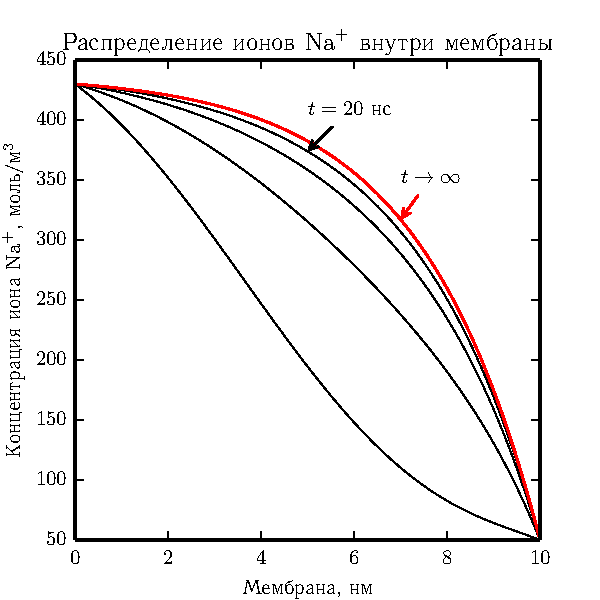
\includegraphics[width=.7\textwidth]{plots/linear_field}
    \end{center}
    \caption{Процесс установления профиля концентрации в постоянном поле. Чёрные
    кривые -- профили в различные моменты времени с шагом 5 нс, красная --
    установившийся профиль.}
    \label{fig:1}
    \end{figure}


\section{Приближение постоянного градиента концентрации}
\subsection{Условие применимости}
    Как и в приближении постоянного поля достаточно потребовать малости поля
    ионов в мембране по сравнению с внешним полем
    \[
        E = \frac{\phi_0}{\ln\frac{c_{out}}{c_{in}}}
            \frac{c_{in} - c_{out}}{d}
            \frac{1}{c_{out} - \frac{c_{out} - c_{in}}{d} x}.
    \]
    Внешнее поле принимает минимальное значение на том краю, где концентрация
    ионов больше:
    \[
        E_{min} = \frac{\phi_0}{\ln\frac{c_{out}}{c_{in}}}
            \frac{c_{in} - c_{out}}{d}\frac{1}{\max(c_{out}, c_{in})}.
    \]
    Для собственного поля ионов имеем
    \begin{gather*}
        E_i(x) = E_i(0) + \frac{Fz}{\eps\eps_0}\int_0^x c(\xi)d\xi = \\
        = E_i(0) + \frac{Fz}{\eps\eps_0}\left(
        c_{out} x - \frac{c_{out} - c_{in}}{d}\frac{x^2}{2}\right).
    \end{gather*}
    Максимальное значение оно принимает на краях мембраны. Поле ионов имеет вид
    \[
        E_i(x) = \frac{Fz}{\eps\eps_0}\left[
        c_{out} \left(x-\frac{d}{2}\right) - \frac{c_{out} - c_{in}}{2d}
        \left(x^2 - \frac{d^2}{2}\right)
        \right].
    \]
    \[
        E_i^{max} = \frac{Fzd}{\eps\eps_0}\frac{c_{in}+c_{out}}{4} \ll E_{min}.
    \]

\subsection{Решение уравнения}
    Уравнение
    \begin{gather*}
        \pder{c}{t} = \frac{uRT}{e|z|}\ppder{c}{x} -
        \frac{z}{|z|}u\frac{\phi_0}{\ln\frac{c_{out}}{c_{in}}}
        \frac{c_{in} - c_{out}}{d}
        \frac{1}{c_{out} - \frac{c_{out} - c_{in}}{d} x}
        \pder{c}{x} + \\
        + \frac{|z|}{z}u\frac{\phi_0}{\ln\frac{c_{out}}{c_{in}}}
        \frac{(c_{in} - c_{out})^2}{d^2}
        \frac{1}{(c_{out} - \frac{c_{out} - c_{in}}{d} x)^2}c.
    \end{gather*}
    можно переписать в виде
    \[
        \pder{c}{t} = D\ppder{c}{x} - vf(x)\pder{c}{x} + \frac{v}{d}f^2(x)c,
    \]
    где
    \[
        D = \frac{uRT}{e|z|},\ v = \frac{z}{|z|}\frac{u}{d}
        \frac{\phi_0}{\ln\frac{c_{out}}{c_{in}}},
        \ f(x) = \frac{d}{x - c_{out}d / (c_{out}-c_{in})}.
    \]
    Это уравнение с переменными коэффициентами, в котором в свою очередь можно
    уйти от конкретных размеров мембраны:
    \[
        \pder{c}{\tau} = \ppder{c}{\xi} - wg(\xi)\pder{c}{\xi} + wg^2(\xi)c,
    \]
    где
    \[
        \tau = \frac{D}{d^2}t,\ \xi = \frac{x}{d},\ w = \frac{vd}{D},
        \ g(\xi) = \frac{1}{\xi - \frac{c_{out}}{c_{out} - c_{in}}}.
    \]
    Поставим для этого уравнения краевую задачу:
    \begin{align*}
        & \pder{c}{\tau} = \ppder{c}{\xi} - wg(\xi)\pder{c}{\xi} + wg^2(\xi)c,
            \ \xi\in(0,1) \\
        & c(0, \tau) = c_{out},\ \tau>0 \\
        & c(1, \tau) = c_{in},\ \tau>0 \\
        & c(\xi, 0) = 0,\ \xi\in(0,1).
    \end{align*}
    Явная разностная схема в этом случае имеет вид:
    \begin{gather*}
        c(\xi_i,\tau_{j+1}) =
        [1-2r+qg^2(\xi)]c(\xi_i, \tau_j) +\\
        + r\left(
            [1 - sg(\xi_i)]c(\xi_{i+1},\tau_j) +
            [1 + sg(\xi_i)]c(\xi_{i-1},\tau_j)
        \right),\\
        r = \frac{\Delta\tau}{\Delta\xi^2}, s = \frac{w\Delta\xi}{2},
        q = w\Delta\tau.
    \end{gather*}
    Результат численного решения для иона натрия в мембране аксона кальмара
    представлен на рисунке~\ref{fig:2}.
    \begin{figure}[H]
    \begin{center}
        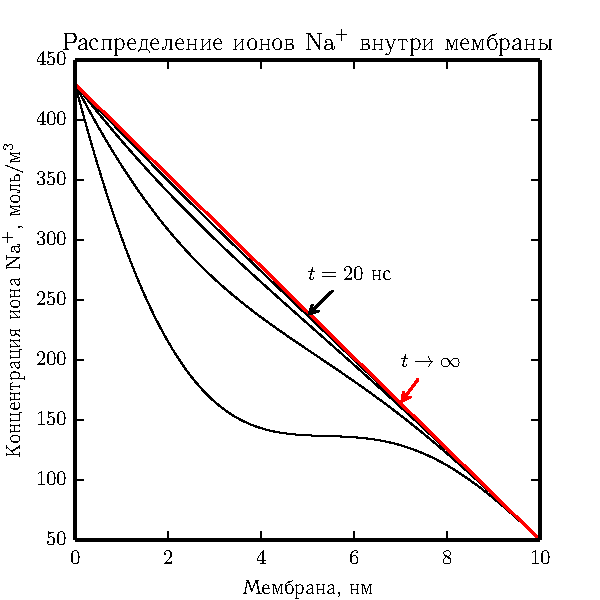
\includegraphics[width=.6\textwidth]{plots/linear_conc}
    \end{center}
    \caption{Процесс установления линейного профиля концентрации. Чёрные кривые
    -- профили в различные моменты времени с шагом 5 нс, красная --
    установившийся линейный профиль.}
    \label{fig:2}
    \end{figure}

    Таким образом, за время порядка \(10^{-8}\) -- \(10^{-7}\) с в обоих
    рассмотренных приближениях устанавливается равновесное распределение
    концентраций.

\section{Учёт поля ионов}
    Запишем снова уравнение Нернста-Планка:
    \[
        j = -\frac{z}{|z|}uRT\pder{c}{x} + |z|cuFE.
    \]
    Поле \( E \) складывается из нескольких компонент: внешнего поля и полей,
    создаваемых каждым из сортов ионов в мембране.
    \[
        E = E_{ex} + \sum_{i} E_i.
    \]
    Рассмотрим случай пассивного транспорта ионов одного сорта. В этом случае
    \[
        E = E_{ex} + E_{in}.
    \]
    Так как задача плоская, то внешнее поле может быть только однородным.
    Электрическое поле ионов связано с их концентрацией уравнением Максвелла:
    \[
        \pder{E_{in}}{x} = \frac{cFz}{\eps\eps_0},\quad
        c = \frac{\eps\eps_0}{Fz}\pder{E_{in}}{x}.
    \]
    Тогда плотность ионного тока определяется выражением
    \begin{equation}
        j = \eps\eps_0
            \left(-D_i\ppder{E_{in}}{x}+
            \frac{z_i}{|z_i|}u_iE\pder{E_{in}}{x}\right).
        \label{eq:j_from_E}
    \end{equation}
    Теперь воспользуемся уравнением непрерывности:
    \[
        \pder{\rho}{t} + \pder{j}{x} = 0.
    \]
    Выразим плотность заряда из уравнения Максвелла и подставим в уравнение
    непрерывности:
    \[
        \pder{E_{in}}{x} = \frac{\rho}{\eps\eps_0},\quad
        \eps\eps_0\pder{}{t}\pder{E_{in}}{x} + \pder{j}{x} = 0.
    \]
    Отсюда
    \[
        \pder{}{x}\left(\eps\eps_0\pder{E_{in}}{t} + j\right) = 0,
    \]
    \begin{equation}
        \pder{j}{x} = -\eps\eps_0\pcder{E_{in}}{x}{t}.
        \label{eq:displacement-current}
    \end{equation}
    Подставляя \eqref{eq:displacement-current} в \eqref{eq:j_from_E}, получаем
    нелинейное дифференциальное уравнение третьего порядка для поля:
    \begin{equation}
        \pcder{E}{x}{t} = D\frac{\partial^3{E}}{\partial x^3} -
        \frac{z}{\abs{z}}\frac{u}{2}\ppder{E^2}{x}.
        \label{eq:epic-equation}
    \end{equation}
    Граничное условие для неё можно поставить в виде
    \[
        \left.\pder{E}{x}\right|_{x=0} = \frac{Fz}{\eps\eps_0}c(0),\quad
        \left.\pder{E}{x}\right|_{x=d} = \frac{Fz}{\eps\eps_0}c(d).
    \]
    Интегрируя \eqref{eq:epic-equation}, получаем
    \begin{equation}
        \pder{E}{t} = D\ppder{E}{x} -
        \frac{z}{\abs{z}}\frac{u}{2}\pder{E^2}{x} - C_1(t).
        \label{eq:epic-integrated}
    \end{equation}
    В стационарном процессе
    \[
        \pder{E}{t} = 0,\quad C_1(t) = C_1,
    \]
    поэтому уравнение можно проинтегрировать ещё раз:
    \[
        D\pder{E}{x} - \frac{z}{\abs{z}}\frac{u}{2}E^2 = C_1 x + C_2.
    \]
    Однако, так как уравнение \eqref{eq:epic-equation} является уравнением
    третьего порядка по пространственной координате, то для нахождения решения
    необходимы 3 граничных условия. Так как в нашем распоряжении только 2
    граничных условия, то задача не может быть решена. Если же найти
    недостающее граничное условие, то решив это уравнение можно получить и
    распределение концентраций
    \[
        c(x) = \frac{\eps\eps_0}{Fz}\pder{E}{x},
    \]
    и плотность тока ионов, подставив полученные зависимости в уравнение
    Нернста--Планка~\eqref{eq:nernst-plank-2}.

\section{Воздействие СВЧ-поля на мембранный транспорт}
    Рассмотрим действие СВЧ-поля на мембранный транспорт. Пусть в мембране
    установился стационарный режим, при этом поле в мембране \( E^{(0)}(x) \).
    Поместим теперь мембрану во внешнее поле \( E_m e^{i\omega t} \), причём
    \( \abs{E_m} \ll E^{(0)} \). СВЧ-поле внесёт возмущение в распределение
    ионов в мембране и, как следствие, в распределение поля. Поэтому
    результирующее поле можно представить в виде
    \begin{equation}
        E = E_m e^{i\omega t} + E^{(0)} + E^{(1)} + \ldots
    \end{equation}
    Подставим это поле в полученное ранее уравнение \eqref{eq:epic-equation}:
    \begin{gather*}
        \pcder{\left(E_m e^{i\omega t} + E^{(0)} + E^{(1)}\right)}{x}{t} =
         D\frac{\partial^3
             \left(E_m e^{i\omega t} + E^{(0)} + E^{(1)}\right)
        }{\partial x^3}
         -\\-
        \frac{z}{\abs{z}}u\pder{}{x}\left[
        \left(E_m e^{i\omega t} + E^{(0)} + E^{(1)}\right)
        \pder{\left(E_m e^{i\omega t} + E^{(0)} + E^{(1)}\right)}{x}\right].
    \end{gather*}
    Так как стационарное поле \( E^{(0)} \) так же удовлетворяет этому
    уравнению, а \( E_m = \const \), то уравнение можно упростить, оставив при
    этом только величины первого порядка малости:
    \begin{gather*}
        \pcder{E^{(1)}}{x}{t} = D\frac{\partial^3 E^{(1)}}{\partial x^3} +
        \frac{uzE^{(0)}}{\abs{z}}\ppder{E^{(1)}}{x} +
        2\frac{uz}{\abs{z}}\pder{E^{(0)}}{x}\pder{E^{(1)}}{x} + \\ +
        \frac{uz}{\abs{z}}\ppder{E^{(0)}}{x} E^{(1)} +
        \frac{uz}{\abs{z}}\ppder{E^{(0)}}{x} E_m e^{i\omega t}.
    \end{gather*}
    Это линейное дифференциальное уравнение в частных производных третьего
    порядка с переменными коэффициентами.

    Также возможен другой подход. Представим поле в мембране в виде
    \( E = E_0 + E_1e^{i\omega t} \), где \( E_0 \) -- постоянная составляющая,
    соответствующая установившемуся процессу в мембране, а \( E_1e^{i\omega t} \)
    -- переменная, отвечающая за СВЧ-воздействие. Тогда подставив эту сумму в
    уравнение \eqref{eq:epic-integrated} учётом того, что \( E_0 \)
    удовлетворяет этому уравнению, получим
    \[
        i\omega E_1 = D\ppder{E_1}{x} - \frac{uz}{\abs{z}}\pder{E_0}{x}E_1.
    \]
    При этом, считая, что концентрации
    ионов в омывающих растворах не изменяются, можно получить граничное условие:
    \[
        \left.\pder{E_1}{x}\right|_{x=0} = \left.\pder{E_1}{x}\right|_{x=d} = 0.
    \]
    Это линейное уравнение второго порядка может быть решено при известном
    распределении поля \( E_0 \) в мембране. Но, по приведённым выше причинам,
    получить выражение для \( E_0 \) пока не представляется возможным.

\newpage
\begin{center}
    ЗАКЛЮЧЕНИЕ
\end{center}
\addcontentsline{toc}{chapter}{Заключение}
В данной работе была предпринята попытка получить эквивалент уравнения
Нернста—Планка для нестационарного процесса. Было получено уравнение
\eqref{eq:nernst-plank-2_with_time}, которое может быть использовано для рассмотрения
нестационарного процесса переноса ионов в мембране, однако его недостатком является то,
что для его решения требуется явный вид профиля потенциала в мембране.
В качестве попытки обойти эту проблему, было получено уравнение
\eqref{eq:epic-equation}, которое включает в себя только одну неизвестную функцию.
Но и это уравнение в том виде, в котором оно получено, не может решить
поставленную задачу, так как для постановки краевой задачи требуется 3
граничных условия, в то время как у нас имеется только 2. Тем не менее,
если удастся решить эту проблему, то данное уравнение можно будет
использовать для описания транспорта ионов в мембране при наличии
высокочастотного поля.

\newpage
\addcontentsline{toc}{chapter}{Список использованных источников}
\def\bibname{СПИСОК ИСПОЛЬЗОВАННЫХ ИСТОЧНИКОВ}
\begin{thebibliography}{99}
\bibitem{bib:1} Шеин, А. Г. Математические модели влияния СВЧ-излучения низкой
    интенсивности на пассивный транспорт ионов : монография / А. Г. Шеин, Н. В.
    Грецова ; ВолгГТУ.~--- Волгоград : ИУНЛ ВолгГТУ, 2012.~--- 148 c.
\bibitem{bib:2} The influence of microwave radiation from cellular phone on
    fetal rat brain~/ J. Jing [et al] // Electromagnetic Biology and
    Medicine.~--- 2012.~--- Vol. 31, № 1~--- P.~57--66.
\bibitem{bib:3} Шеин, А. Г. Токи через мембрану с учетом наличия высокочастотных
    составляющих / А. Г. Шеин, Д. А. Барышев // Биомедицинская радиоэлектроника.~---
    2009.~--- №~4.~--- С. 4--9.
\bibitem{bib:4} Warchalewski, J. R. Influence of microwave
    heating on biological activities and electrophoretic pattern of
    albumin fraction of wheat grain /  J. R. Warchalewski, J. Gralik //
    СerealСhemistry.~--- 2010.~--- Vol. 87, № 1.~--- P.~35--41.
\bibitem{bib:5} Исмаилов, Э. Ш. Биофизическое действие СВЧ-излучений / Э. Ш.
    Исмаилов.~--- Москва : Энергоатомиздат, 1987.~--- 144 с.
\bibitem{bib:6} Тамбиев, А. Х. Влияние КВЧ-излучения на транспортные свойства
    мембран у фотосинтезирующих организмов / А. Х. Тамбиев, Н. Н. Кирикова,
    Е. Н. Маркарова // Биомедицинская радиоэлектроника.~--- 1997.~--- №~4.~--- С.
    67--76.
\bibitem{bib:7} Чопчиян, А. С. О краевых задачах для уравнений Нернста--Планка
    и Пуассона / А. С. Чопчиян, Е. Н. Коржов // Системы управления и
    информационные технологии.~--- 2009.~--- №~38.~--- С. 200--203.
\bibitem{bib:8} Маркин, В. С. Индуцированный ионный транспорт / В. С. Маркин,
    Ю. А. Чизмаджев.~--- Москва : Наука, 1974.~--- 252 с.
\bibitem{bib:9} Рубин, А. Б. Биофизика. В 2 т. Т. 2. Биофизика клеточных
    процессов / А. Б. Рубин.~--- Москва : Высшая школа, 1999.~--- 464 с.
\bibitem{bib:10} Биофизика : учебник для студентов вузов / В. Ф. Антонов [и др.] ;
    под ред. Антонова.~--- 3-е изд., испр. и доп.~--- Москва : Владос, 2006.~--- 287 с.
\bibitem{bib:11} Hille, B. Ion channels of excitable membranes / B.
    Hille.~--- 3rd ed.~--- Sunderland : Sinauer Associates, 2001.~--- 814 p.
\bibitem{bib:12} Плонси, Р. Биоэлектричество: Количественный подход / Р. Плонси,
    Р. Барр.~--- Москва : Мир, 1992.~--- 366 c.
\bibitem{bib:13} Биофизика / П. Г. Костюк [и др.] ; под ред. П. Г. Костюка.~--- Киев: Высшая
    школа, 1988.~--- 504 с.
\bibitem{bib:14} Иваницкий, Г. Р. Математическая биофизика клетки / Г. Р.
    Иваницкий, В. И. Кринский, Е. Е. Сельков.~--- Москва : Наука, 1987.~---
    308 c.
\bibitem{bib:15} Лев, А. А. Ионная избирательность клеточных мембран /
    А. А. Лев.~--- Ленинград : Наука, 1975.~--- 323 с.
\bibitem{bib:16} Антонов, В. Ф. Биофизика мембран / В. Ф. Антонов // Соросовский
    образовательный журнал.~--- 1996.~--- №~6.~--- С. 1--15.
\bibitem{bib:17} Боровягин, В. Л. Клеточные мембраны / В. Л. Боровягин //
    Биологические мембраны.~--- 1971.~--- №~4.~--- С. 746--766.
\bibitem{bib:18} Жулев, В. И. Исследование электрических процессов в клеточных
    структурах / В. И. Жулев, И. А Ушаков // Биомедицинская электроника.~---
    2001.~--- №~7.~--- С. 30--37.
\bibitem{bib:19} Кудряшов, Ю. Б. Биофизические основы действия микроволн /
    Ю. Б. Кудряшов, Э. Ш. Исмаилов, С. М. Зубкова.~--- Москва : МГУ, 1980.~---
    160 с.
\end{thebibliography}

\end{document}
